\section{文献检索、阅读与汇报}

\subsection{检索渠道}
\begin{itemize}
  \item 中文入门：知网优质综述（适应英文前可先建立领域地图）。
  \item 英文主渠道：Google Scholar、\texttt{arxiv.org}、AMiner（\url{https://www.aminer.cn/}）、PubScholar（\url{https://pubscholar.cn/}）。
  \item 代码与论文绑定：Papers with Code（\url{https://paperswithcode.com/}）。
  \item 引用关系可视化：Connected Papers、Open Knowledge Maps（\url{https://openknowledgemaps.org/}）。
  \item 会议/期刊权威性：参考 CCF 列表；组内常用投稿目标见图~\ref{fig:journal-list}。
\end{itemize}

\begin{figure}[htbp]
  \centering
  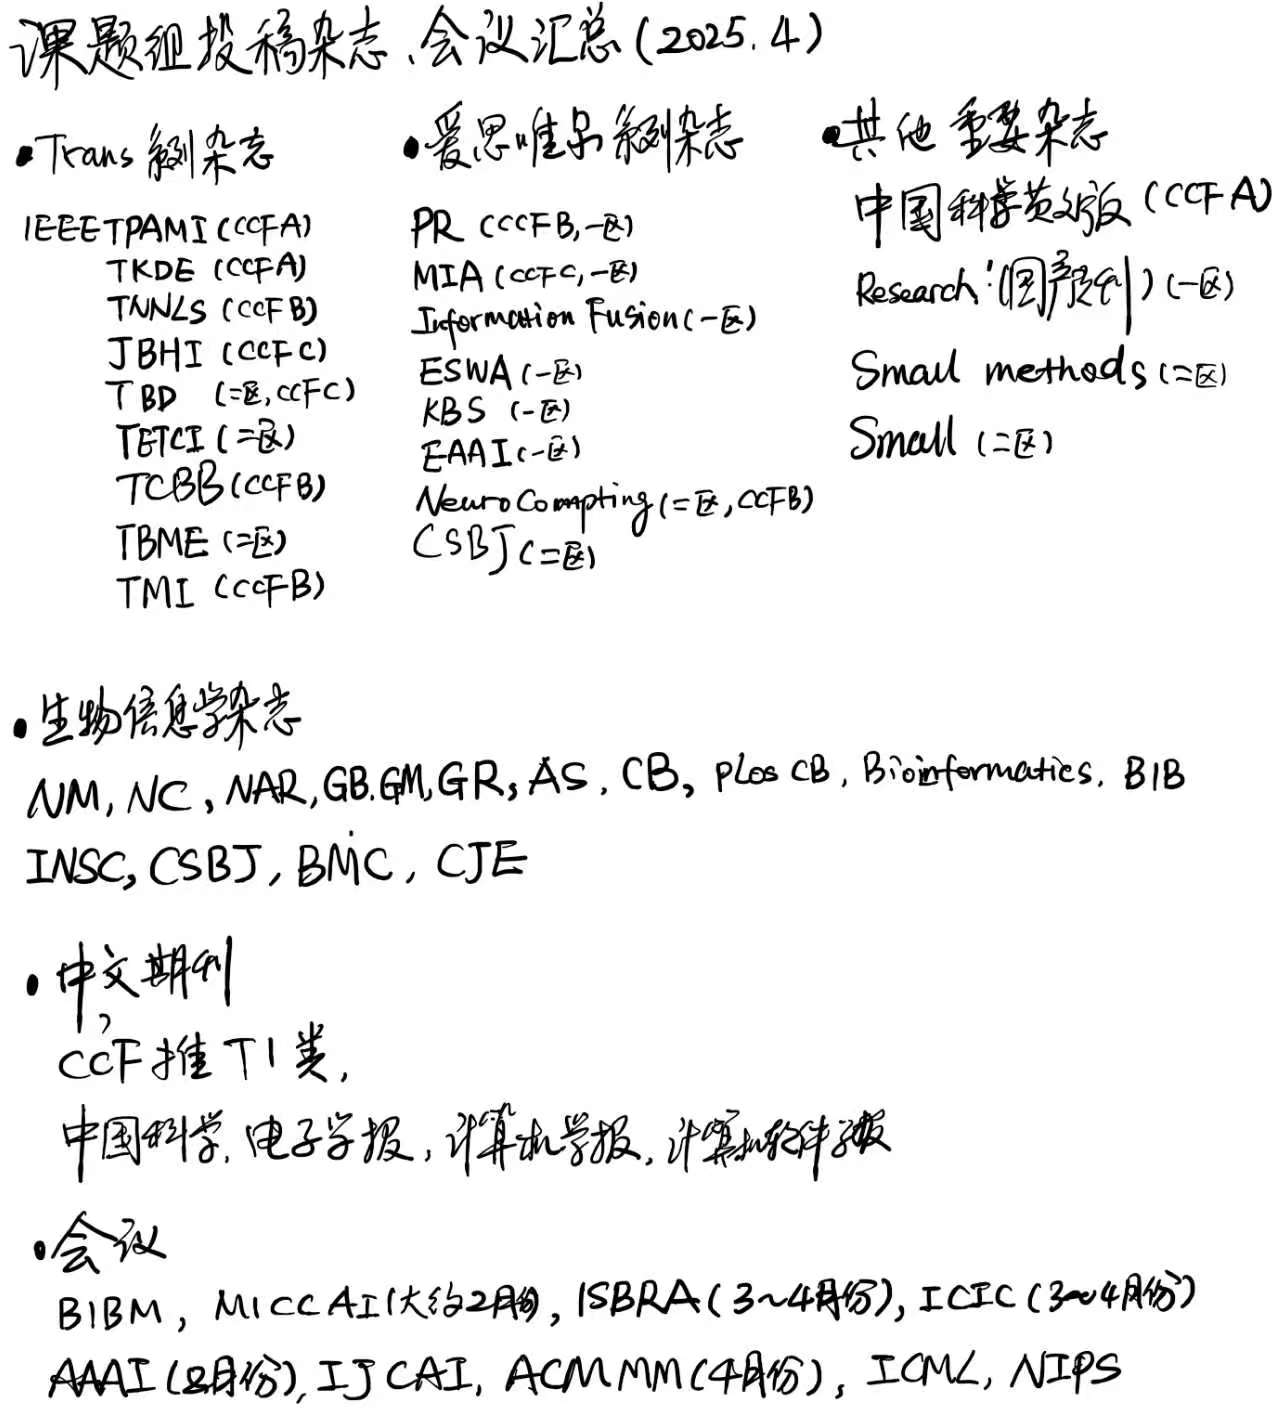
\includegraphics[width=0.92\textwidth]{figures/journal_list.jpg}
  \caption{课题组投稿期刊/会议汇总示意（以组内最新版本为准）}
  \label{fig:journal-list}
\end{figure}

\subsection{优先关注的顶刊顶会入口}
调研相关工作时，优先从以下来源筛选（完整链接见第~8~章）：
PR、IEEE TPAMI、TIP、IEEE TNNLS、AAAI、CVPR、ECCV、ICCV、ACM MM、NeurIPS 等。
常用开放获取入口示例：
\begin{itemize}
  \item CVPR 2024：\url{https://openaccess.thecvf.com/CVPR2024}
  \item ECCV：\url{https://www.ecva.net/papers.php}
  \item ICCV：\url{https://openaccess.thecvf.com/ICCV2023}
  \item TIP / TPAMI：IEEE Xplore 期刊近期论文页
\end{itemize}

\subsection{文献筛选策略}
\begin{enumerate}
  \item 先读\textbf{英文综述}：主流方法、开放问题、数据集、指标、前景。
  \item 再筛论文：经典 / 顶会顶刊 / 有代码有数据者优先；无代码也可借鉴思想与 trick。
  \item 看不懂时：知乎、B 站、油管上的论文/代码解读可作辅助，但结论需回原文核对。
\end{enumerate}

\subsection{建立文献 List（强制习惯）}
每条记录建议至少包含：题目、作者、引用量、发表时间、链接、有无代码及链接、有无数据集及链接。
可复制仓库模板：\path{templates/literature_list.csv}；范例清单见 \path{assets/reading-list/}。

\subsection{阅读顺序与精读目标}
\textbf{泛读顺序：} Abstract + 文中第一张总览图 $\rightarrow$ Introduction $\rightarrow$ Conclusion；\\
确有继续价值再读 Method $\rightarrow$ Experiment。

精读一篇后，应能讲清：
\begin{itemize}
  \item 问题定义（输入/输出、指标、数据）；
  \item 背景与现有方法不足；
  \item 研究动机与方法框架；
  \item 主要实验结论与 contribution；
  \item 对你课题的可迁移点。
\end{itemize}
\tipbox{读第一篇领域论文不要过于乐观，真正读懂常需 1--2 周；读懂一篇往往要连带读十余篇相关工作，这是正常现象。}

文献管理推荐：Zotero（可配合坚果云同步）。笔记可用 Obsidian / Notion。

\subsection{论文汇报 Checklist}
汇报一篇论文时，建议覆盖：
\begin{enumerate}
  \item Background：为什么有必要做；
  \item Challenge：技术/应用难点；
  \item Existing methods：已有路线与不足；
  \item Method：核心思路与框架图；
  \item Dataset \& metrics；
  \item Results：对比与消融；
  \item Conclusion + 你的批判性思考与下一步。
\end{enumerate}
扫描版要点图册见仓库 \texttt{assets/tips/literature\_and\_report\_tips.pdf}。

\subsection{周汇报 Checklist}
\begin{itemize}
  \item 上周遗留问题是否解决；
  \item 本周具体工作（文献/代码/实验/写作）；
  \item 本周卡点与已尝试的排查；
  \item 下周计划与需要的支持。
\end{itemize}
模板：\texttt{templates/weekly\_report.md}。
